\documentclass[rpussian]{beamer}

\usepackage{cmap} % для кодировки шрифтов в pdf
\usepackage[T2A]{fontenc}
\usepackage[utf8]{inputenc}
\usepackage[russian]{babel}
\usepackage{minted} % code highlighting

\usepackage{graphicx} % для вставки картинок
\graphicspath{ {img/} }

%\usetheme{Rochester}
\usecolortheme{wolverine}
\definecolor{bg}{rgb}{0.95,0.95,0.95}

\newcommand\imagesthree[6]{
  \begin{columns}[b]
    \begin{column}{.5\textwidth}
      \begin{center}
        \includegraphics[width=4cm,keepaspectratio]{#1}
        \newline
        \scriptsize #2
      \end{center}
    \end{column}
    \begin{column}{.5\textwidth}
      \begin{center}
      \includegraphics[width=4cm,,keepaspectratio]{#3}
      \newline
      \scriptsize #4
      \end{center}
    \end{column}
  \end{columns}
  \begin{center}
    % Hack. Don't know why image is shifted to left a bit by default.
    \hspace*{1.2cm} \includegraphics[width=4cm,keepaspectratio]{#5}
    \newline
    \scriptsize #6
  \end{center}
}

\title[Интерполяция]{Алгоритмы интерполяции функций.\newline Создание библиотеки на языке Clojure.}
\author{Белоглазов Никита}
\date{2013}
\institute{Белорусский Государственный Университет}

\begin{document}

\maketitle
\begin{frame}[fragile]
  \frametitle{Clojure}
  \begin{minted}[bgcolor=bg,gobble=4,frame=single]{clojure}
    (defn derivative [f x]
      (let [h 0.00001]
        (/ (- (f (+ x h))
              (f x))
           h)))

    (defn f1 [x] x)       ; f1(x) = x
    (defn f2 [x] (* x x)) ; f2(x) = x * x

    (derivative f1 0) ; 1
    (derivative f2 0) ; 0.00001
    (derivative f2 4) ; 8.00001
  \end{minted}
\end{frame}

\begin{frame}
  \frametitle{Incanter}

  \emph{Incanter} - математический R-подобный пакет для алгебраических и статистических расчётов на языке Clojure.

  \begin{itemize}

  \item Функции для построения графиков и визуализации данных.

  \item Математические функции.

  \item Статистические функции.

  \item Функции для работы с матрицами и линейной алгеброй.

  \item Функции обработки данных.

  \item \emph{Функции построения интерполирующих функций.}
  \end{itemize}
\end{frame}

\begin{frame}
  \frametitle{Интерполяция}
  \begin{center}
    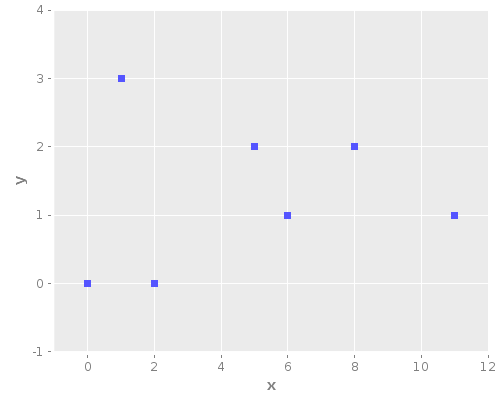
\includegraphics[width=.4\textwidth,height=.4\textheight,keepaspectratio]{points}
    \\
    ?
  \end{center}
  \begin{columns}[c]
    \begin{column}{.35\textwidth}
      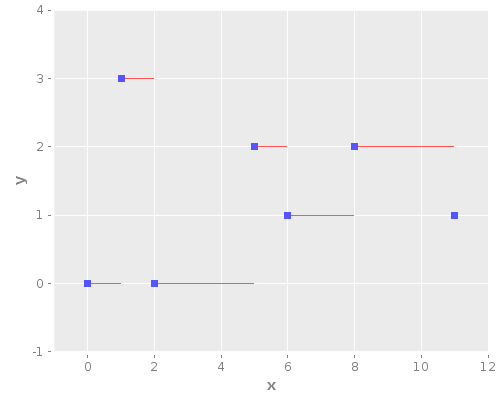
\includegraphics[width=\textwidth,height=\textheight,keepaspectratio]{interrupted}
    \end{column}
    \begin{column}{.35\textwidth}
      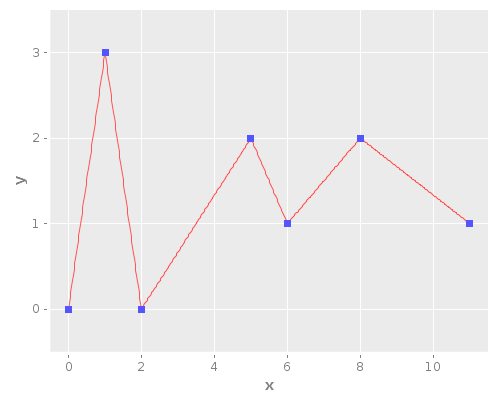
\includegraphics[width=\textwidth,height=\textheight,keepaspectratio]{linear_interpolation_1_var_small}
    \end{column}
    \begin{column}{.35\textwidth}
      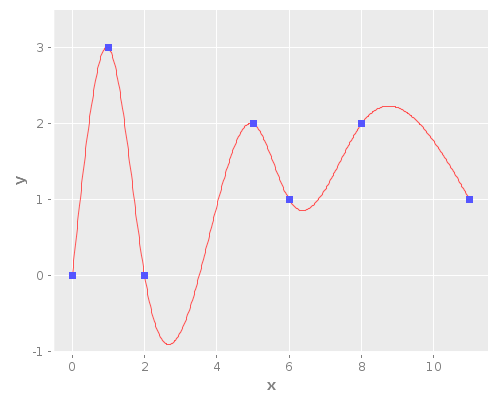
\includegraphics[width=\textwidth,height=\textheight,keepaspectratio]{cubic_interpolation_1_var_small}
    \end{column}
  \end{columns}
\end{frame}

\begin{frame}[fragile]
  \frametitle{API}
  \verb+(interpolate points type & options)+ \\
  строит $f(x) = y$, проходящую через точки $(x, y)$ \\

  \vspace{1.2cm}

  \verb+(interpolate-parametric points type & options)+ \\
  строит $f(t) = (x_1, ..., x_n)$, задающую кривую, проходяющую через точки $(x_1, ..., x_n)$ \\

  \vspace{1.2cm}

  \verb+(interpolate-grid grid type & options)+ \\
  строит $f(x, y) = z$, по прямоугольной сетке
\end{frame}

\begin{frame}[fragile]
  \frametitle{interpolate}
  \verb+(interpolate points type & options)+ \\
  \vspace{0.5cm}
  Интерполяция: линейная, полиномиальная, кубический сплайн, кубический эрмитов сплайн, среднеквадратичное приближение.
  \vspace{0.5cm}
  \begin{minted}[bgcolor=bg,gobble=4,frame=single]{clojure}
    (def points [[0 0] [1 3] [2 0] [4 2]])

    (def cubic (interpolate points :cubic
                            :boundaries :closed))

    (cubic 0) ; 0.0
    (cubic 1) ; 3.0
    (cubic 3) ; -1.2380952380952381
  \end{minted}
\end{frame}

\begin{frame}
  \frametitle{interpolate примеры}
  \imagesthree
  {linear_interpolation_1_var_small}{Линейная интерполяция\\ \hspace*{5cm}} % Hack need to span caption over 2 lines.
  {lls_polynomial_3_1_var_small}{Среднеквадратичное приближение по базису $(1, x, x^2)$}
  {lls_sin_1_var_small}{Среднеквадратичное приближение по базису $(1, x, x^2, sin(x))$}
\end{frame}

\begin{frame}
  \frametitle{interpolate примеры}
  \imagesthree
  {cubic_interpolation_1_var_small}{Кубический сплайн}
  {cubic_hermite_interpolation_1_var_small}{Кубический эрмитов сплайн}
  {polynomial_interpolation_1_var_small}{Полиномиальная интерполяция}
\end{frame}



\begin{frame}[fragile]
  \frametitle{interpolate-parametric}
  \verb+(interpolate-parametric points type & options)+ \\
  \vspace{0.5cm}
  Интерполяция: линейная, полиномиальная, кубический сплайн, кубический эрмитов сплайн, среднеквадратичное приближение, B-сплайн.
  \vspace{0.5cm}
  \begin{minted}[bgcolor=bg,gobble=4,frame=single]{clojure}
    (def points [[0 0] [1 3] [2 0] [4 2]])

    (def linear (interpolate-parametric points :linear
                                        :range [-1 1]))

    (linear -1) ; (0.0 0.0)
    (linear  1) ; (4.0 2.0)
    (linear  0) ; (1.5 1.5)
  \end{minted}
\end{frame}

\begin{frame}
  \frametitle{interpolate-parametric примеры}
  \imagesthree
  {linear_parametric_interpolation_small}{Линейная интерполяция\\ \hspace*{5cm}} % Hack. Need to span caption over 2 lines.
  {lls_polynomial_parametric_4_small}{Среднеквадратичное приближение по базису $(1, x, x^2, x^3)$}
  {b_spline_parametric_small}{B-сплайн 3 степени}
\end{frame}

\begin{frame}
  \frametitle{interpolate-parametric примеры}
  \imagesthree
  {cubic_closed_parametric_interpolation_small}{Кубический сплайн}
  {cubic_hermite_parametric_interpolation_small}{Кубический эрмитов сплайн}
  {polynomial_parametric_interpolation_small}{Полиномиальная интерполяция}
\end{frame}

\begin{frame}[fragile]
  \frametitle{interpolate-grid}
  \verb+(interpolate-grid grid type & options)+ \\
  \vspace{0.5cm}
  Интерполяция: билинейная, полиномиальная, бикубический сплайн, бикубический эрмитов сплайн, B-сплайновая поверхность.
  \vspace{0.5cm}
  \begin{minted}[bgcolor=bg,gobble=4,frame=single]{clojure}
    (def grid [[0 1 2]
               [3 4 5]
               [6 7 8]])

    (def bilinear (interpolate-grid grid :bilinear))

    (bilinear    0   0) ; 0.0
    (bilinear    1   1) ; 8.0
    (bilinear  0.5 0.5) ; 4.0
    (bilinear 0.25   1) ; 6.5
  \end{minted}
\end{frame}

\begin{frame}
  \frametitle{interpolate-grid примеры}
  \imagesthree
  {small_bilinear}{Билинейная интерполяция}
  {small_b_surface}{B-сплайновая поверхность}
  {small_polynomial}{Полиномиальная интерполяция}
\end{frame}

\begin{frame}
  \frametitle{interpolate-grid примеры}
    \begin{columns}[c]
    \begin{column}{.5\textwidth}
      \begin{center}
        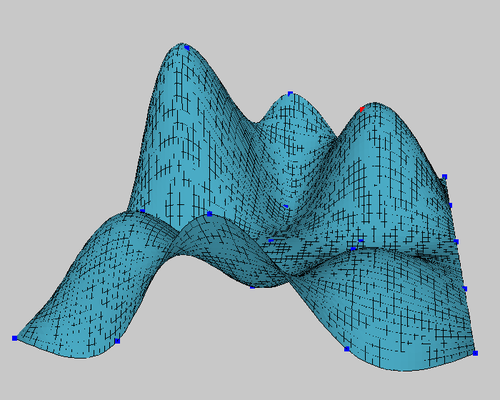
\includegraphics[width=\textwidth,keepaspectratio]{small_bicubic}
        \newline
        \scriptsize Бикубический сплайн
      \end{center}
    \end{column}
    \begin{column}{.5\textwidth}
      \begin{center}
      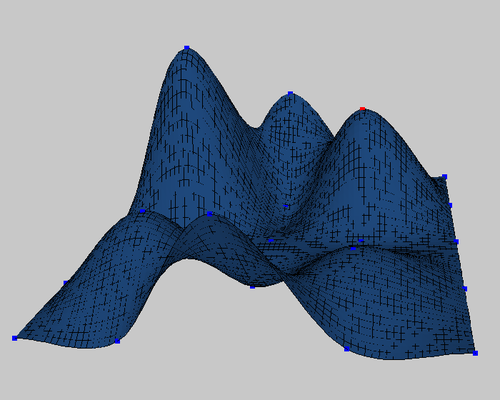
\includegraphics[width=\textwidth,keepaspectratio]{small_bicubic_hermite}
      \newline
      \scriptsize Бикубический эрмитов сплайн
      \end{center}
    \end{column}
  \end{columns}
\end{frame}

\begin{frame}
  \frametitle{Конец}
  \begin{columns}[c]
    \begin{column}{.5\textwidth}
      \begin{center}
        Спасибо за внимание!
        \\ \vspace{1cm}
        Вопросы?
      \end{center}
    \end{column}
    \begin{column}{.5\textwidth}
      
\includegraphics[width=\textwidth,keepaspectration]{alien}
    \end{column}
  \end{columns}
\end{frame}

\end{document}

%%% Local Variables:
%%% mode: latex
%%% TeX-master: t
%%% End:
